\section{GloVe} \label{sec:Glove}

The \textbf{Global Vectors for Word Representation (GloVe)} model is an unsupervised learning algorithm that aims to capture meaning in a semantic vector space using global count statistics instead of local context (Pennington et al., 2014). GloVe uses probability ratios to represent meaning as vector offsets. 



\subsection{Problem with Word2Vec: Secret in the Loss Function} \label{sec:ProblemWord2VecFromGloveStandpoint}

\nameref{sec:Word2Vec} uses only local and not global context. So even though words ``the" and ``cat" might be used together frequently, \nameref{sec:Word2Vec} will not discern if this is because ``the" is a common word or because ``the" and ``cat" are actually correlated (Kurita, 2018). 

From Pennington et al. (2014), \nameref{sec:Word2Vec} implicitly optimizes over a co-occurrence matrix while streaming over input sentences. In doing so, it optimizes its log likelihood loss of seeing words \emph{simultaneously} in the same context windows, resulting in an alternative way in \cref{eq:Word2VecLossFunction} of expressing \nameref{sec:Word2Vec}'s loss function. 

\begin{equation} 
J = - \sum_i X_i \sum_j P_{ij} \text{log}(Q_{ij}) 
\label{eq:Word2VecLossFunction}
\end{equation} 

In \cref{eq:Word2VecLossFunction}, $X_i = \sum_k X_{ik}$ is the total number of words appearing in the context of word $i$ and $Q_{ij}$ is the probability that word $j$ appears in context of word $i$ and is estimated as $Q_{ij} = \text{softmax} \Big( w_i \cdot w_j \Big)$. Evidently, \nameref{sec:Word2Vec}'s loss function is form of cross entropy between the predicted and actual word distributions found in context of word $i$. The problem with this is twofold: (1) cross entropy models long-tailed distributions poorly, and (2) the cross-entropy here is weighted by $X_i$, causing equal-streaming over data, so a word appearing $n$ times contributes to the loss $n$ times (Pennington et al., 2014). Recognizing there is no inherent justification for streaming across all words equally, GloVe instead computes differences between unnormalized probabilities, contrary to \nameref{sec:Word2Vec} (Kurita, 2018a). 


\subsection{Motivation for GloVe} \label{sec:MotivationGlove}

Previous global count models like Latent Semantic Analysis (LSA) produced word embeddings lacking vector analogical properties and lacking \emph{dimensions of meaning} such as gender, grammar tense, and plurality, disabling downstream models from easily extracting meaning from those word vectors (Kurita, 2018a). Building from past failures while avoiding \nameref{sec:Word2Vec}'s local \hyperref[sec:ProblemWord2VecFromGloveStandpoint]{context problems}, GloVe instead uses a principled and explicit approach for learning these \emph{dimensions of meaning}.


\subsection{Describing GloVe} \label{sec:DefGlove}

%\subsubsection{Notation in GloVe}

%Let $X$ be the matrix of word co-occurrence counts; let $X_{ij}$ be the $ij$-th entry $X$ that counts how many times any word appears in the context of word $i$, and let $P_{ij} = p_{\text{co}} \Big(w_j \; | \; w_i \Big) = \frac {X_{ij}} {X_i}$ be the probability that word $j$ appears in the context of word $i$ (Pennington et al., 2014; Weng, 2017).

\subsubsection{Meaning Extraction Using Co-Occurrence Counts}

GloVe uses a co-occurrence matrix that describes how words co-occur within a fixed sliding window, assuming co-occurrence counts reveal word meaning. Words \textbf{co-occur} when they appear together within this fixed window (Kurita, 2018a). GloVe takes the matrix as input, rather than the entire corpus, so GloVe disregards sentence-level information while taking into account only corpus-wide co-occurrence. 

From Weng (2017), the co-occurrence probability is defined as: 
$$
p_{\text{co}} \Big(w_k \; | \; w_i \Big) = \frac{C(w_i, w_k)}{C(w_i)}
$$
where $C(w_i, w_k)$ counts the co-occurrence between words $w_i$ and $w_k$.  

GloVe's insight is that word meanings are captured by ratios of co-occurrence probabilities rather than the probabilities themselves. To illustrate how GloVe uses these counts, consider two words $w_i =$ ``ice" and $w_j = $ ``steam". 

\begin{itemizeSpaced}{0pt}
    \item \textbf{Case 1:} For context words related to \texttt{ice} but not \texttt{steam} (like \texttt{solid}), the co-occurrence probability $p_{\text{co}} \Big( \texttt{solid} \; | \; \texttt{ice} \Big)$ should be much larger than $p_{\text{co}} \Big( \texttt{solid} \; | \; \texttt{steam} \Big)$, therefore the ratio $\frac {p_{\text{co}} \Big( \texttt{solid} \; | \; \texttt{ice} \Big)} {p_{\text{co}} \Big( \texttt{solid} \; | \; \texttt{steam} \Big)}$ gets very large.

    \item \textbf{Case 2: } Conversely, for words related to \texttt{steam} but not \texttt{ice} (like \texttt{gas}) $\Rightarrow$ the co-occurrence ratio $\frac {p_{\text{co}} \Big( \texttt{gas} \; | \; \texttt{ice} \Big)} {p_{\text{co}} \Big( \texttt{gas} \; | \; \texttt{steam} \Big)}$ should be small. 

    \item \textbf{Case 3:} For words $w$ related to both \texttt{ice} and \texttt{steam} (like \texttt{water}) or related to neither (like \texttt{fashion}), the ratio $\frac {p_{\text{co}} \Big( w \; | \; \texttt{ice} \Big)} {p_{\text{co}} \Big( w \; | \; \texttt{steam} \Big)}$ should be near one. 
\end{itemizeSpaced}


% 
% \subsubsection{Comparing Performance of Word2Vec and GloVe}
% 
% \cref{fig:gloveVsWord2vec} from Pennington et al. (2014) shows that GloVe's learned word embeddings had higher prediction accuracy over both those of \nameref{sec:SkipGram} and \hyperref[sec:CBOW]{CBOW} (using negative sampling) on tasks like \nameref{nlptask:wordanalogy} and \nameref{nlptask:namedentityrecognitionNER}. 
% 
% \begin{figure}[h]
% \vspace{-5pt}
% \centering
% 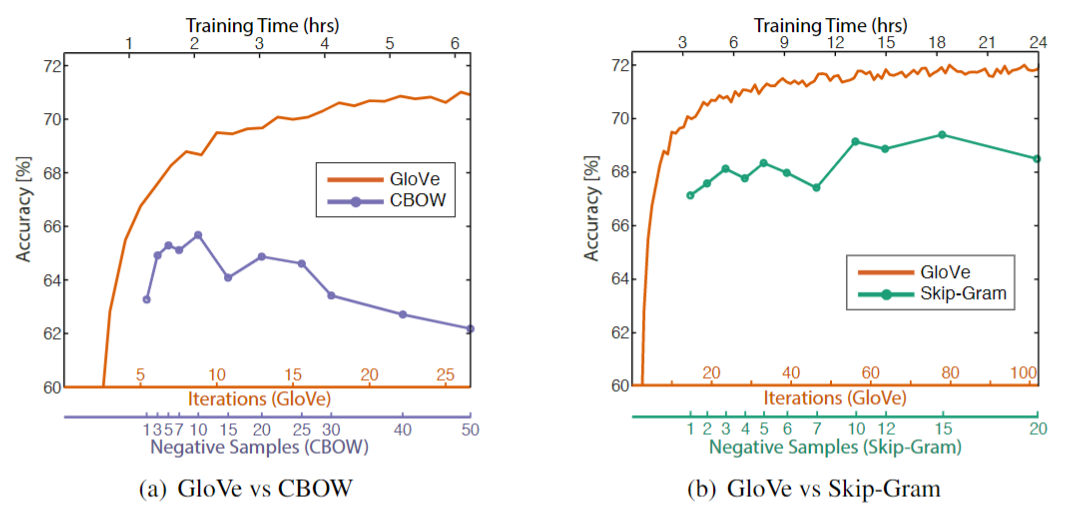
\includegraphics[width=0.65\textwidth]{imgs/table_gloveVSword2vec.png}
% \vspace{-5pt}
% \caption{Overall accuracy on word analogy task as a function of training time, which is governed by the number of iterations for \nameref{sec:Glove} and by the number of negative samples for \hyperref[sec:CBOW]{CBOW} (a) and \nameref{sec:SkipGram} (b). Pennington et al. (2014) train 300-dimensional vectors on the same 6B token corpus from Wikipedia and use a symmetric context window of size 10. From \emph{GloVe: Global Vectors for Word Representation}, by Pennington et al., 2014. \url{https://nlp.stanford.edu/pubs/glove.pdf}. Copyright 2014 by Pennington et al.}
% \vspace{-5pt}
% \label{fig:gloveVsWord2vec}
% \end{figure}